\section{Transactions}

\begin{definition}
    A \emph{transaction} is an elementary, atomic unit of work performed by an application. Each transaction is conceptually encapsulated within two commands:
    \begin{itemize}
        \item Begin transaction.
        \item End transaction.
    \end{itemize}
\end{definition}
Within a transaction, one of the commands below is executed to signal the end of the transaction: commit or rollback. 
\begin{definition}
    The \emph{On-Line Transaction Processing} (OLTP) is a system that supports the execution of transactions on behalf of concurrent applications. 
\end{definition}
The application can run many transactions. So, the transactions are part of the application and not vice-versa. The transactions follow the ACID property: 
\begin{enumerate}
    \item Atomicity: a transaction is an indivisible unit of execution. This means that all the operations in the transaction are executed or none is executed. The time in which 
        commit is executed marks the instant in which the transaction ends successfully: an error before should cause the rollback and an error after should not alter the 
        transaction. The rollback of the work performed can be caused by a rollback statement or by the DBMS. In case of a rollback, the work performed must be undone, bringing 
        the database to the state it had before the start of the transaction. It is the application's responsibility to decide whether an aborted transaction must be redone or not. 
    \item Consistency: A transaction must satisfy the database integrity constraints, that is if the initial state $S_0$ is consistent then the final state $S_f$ is also 
        consistent. This is not necessarily true for the intermediate states $S_i$. 
    \item Isolation: the execution of a transaction must be independent of the concurrent execution of other transactions. 
    \item Durability: the effect of a transaction that has successfully committed will last forever, independently of any system fault. 
\end{enumerate}
\begin{table}[H]
    \centering
    \begin{tabular}{c|c|c}
    \textbf{Property} & \textbf{Actions}       & \textbf{Architectural element} \\ \hline
    Atomicity         & Abort-rollback-restart & Query Manager                  \\
    Consistency       & Integrity checking     & Integrity Control System       \\
    Isolation         & Concurrency control    & Concurrency Control System     \\
    Durability        & Recovery management    & Reliability Manager           
    \end{tabular}
\end{table}
\begin{figure}[H]
    \centering
    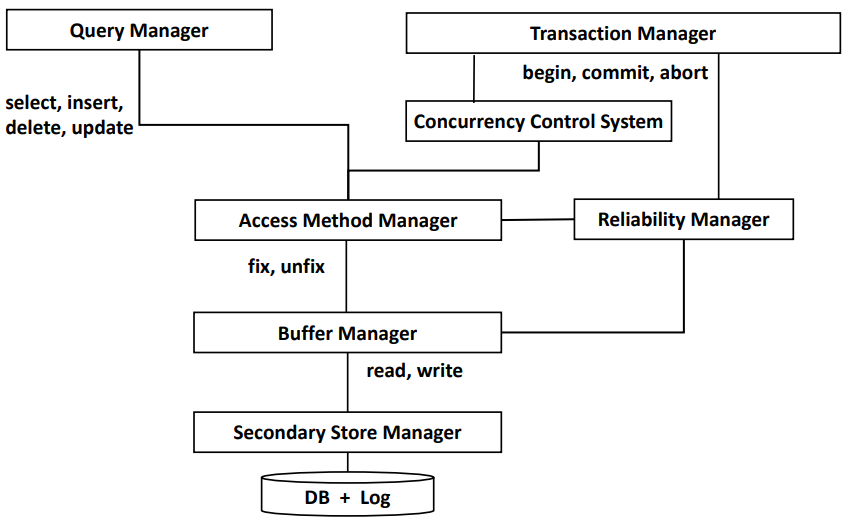
\includegraphics[width=0.75\linewidth]{images/architecture.png}
    \caption{Architecture of a Data Base Management System}
\end{figure}